% =====================================================================
%  Hauptdatei – hier nur Titel, Autor*innen und die Kapitel einbinden.
%  Layout und Pakete stehen in praeambel.tex.
%  Kompilieren:  latexmk main.tex   (nutzt pdflatex + biber, siehe .latexmkrc)
% =====================================================================
\documentclass[
  paper=a4,        % DIN A4
  fontsize=10pt,   % Basis-Schriftgröße (= \normalsize)
  ngerman,
  parskip=half,
  bibliography=totoc,
  listof=totoc,
]{scrreprt}

% =====================================================================
%  Präambel
% =====================================================================

% ---------- Sprache, Kodierung, einheitliche Schrift -----------------
\usepackage[T1]{fontenc}
\usepackage{babel}            % Sprache kommt aus der Klassenoption ngerman
\usepackage{lmodern}          % eine Schriftfamilie für das gesamte Dokument
\usepackage{microtype}
\usepackage[autostyle]{csquotes} % \enquote{...} setzt korrekte „Anführungszeichen“

% KOMA setzt Überschriften standardmäßig serifenlos -> auf Grundschrift umstellen,
% damit überall dieselbe Schriftart verwendet wird.
\setkomafont{disposition}{\normalfont\bfseries}
\setkomafont{caption}{\normalsize}
\setkomafont{captionlabel}{\normalsize\bfseries}

% ---------- Bilder und Tabellen --------------------------------------
\usepackage{graphicx}
\graphicspath{{bilder/}}
\usepackage{booktabs}         % saubere Tabellenlinien
\usepackage{tabularx}
\usepackage{array}
\usepackage{float}
\usepackage[section]{placeins}   % Bilder/Tabellen bleiben in ihrem Abschnitt

% ---------- Literatur: APA 7 ----------------------------------------
\usepackage[style=apa, backend=biber]{biblatex}
\addbibresource{literatur.bib}
\DefineBibliographyStrings{ngerman}{
  nodate      = {o.\,J.},% deutsch „ohne Jahr“
  retrieved   = {Abgerufen am},% deutsch „retrieved“
  from        = {von},% deutsch „at“
}

% ---------- Links und dynamische Verweise ----------------------------
\usepackage[hidelinks]{hyperref}
\usepackage{xurl}             % lange URLs umbrechen
\usepackage[ngerman, noabbrev]{cleveref} % \cref{...} -> „Abbildung 1“, „Tabelle 2“ …

% ---------- Hilfsbefehle ---------------------------------------------
% Quellenangabe für nicht selbst erstellte Bilder, z.\,B. in der Bildunterschrift:
%   \caption{Beschreibung. \bildquelle{schluessel}}
\newcommand{\bildquelle}[1]{(Quelle: \cite{#1})}

% Kennzeichnung von KI-/Automatisierungsnutzung direkt an der betroffenen Stelle:
%   \kihinweis{Tool}{Wofür genutzt}{bib-Schlüssel}
% Beispiel: \kihinweis{ChatGPT}{Gliederungsvorschlag, danach überarbeitet}{openai2026}
\newcommand{\kihinweis}[3]{%
  \footnote{KI-Nutzung: #1 -- #2 \parencite{#3}.}%
}

% Abschnitt „Beiträge“ am Ende jedes Kapitels:
%   \begin{beitraege}
%     Arbeitsschritt/Textteil & Verantwortlich \\
%   \end{beitraege}
\newenvironment{beitraege}{%
  \section{Beiträge}
  \noindent\tabularx{\linewidth}{@{}>{\raggedright\arraybackslash}X >{\raggedright\arraybackslash}p{0.3\linewidth}@{}}
  \toprule
  \textbf{Arbeitsschritt / Textanteil} & \textbf{Verantwortlich} \\
  \midrule
}{%
  \bottomrule
  \endtabularx
}


% --------------------------- Titelangaben ----------------------------
\title{Webanwendung Kanban-Board „tick.it“}
\author{%
  Tara Dethlefsen \and
  Lara Senger \and
  Philipp Wisser%
}
\date{\today}

\begin{document}

\maketitle
\tableofcontents

% Ein Kapitel = eine Aufgabe = eine Datei (weniger Merge-Konflikte)
% =====================================================================
%  Aufgabe 1 – Vorlage für ein Kapitel. Tipp: ein Satz pro Zeile,
%  dann zeigt Git Änderungen satzweise und Konflikte werden seltener.
% =====================================================================
\chapter{Projektthema}
\label{chap:projektthema}

\section{Einleitung}
\label{sec:pt-einleitung}

Im Rahmen dieses Moduls möchten wir die bereits bestehende Webanwendung „tick.it“ weiterentwickeln.
„tick.it“ ist eine Anwendung zur Aufgabenverwaltung, die auf dem Kanban-Prinzip basiert.
Nutzende können Aufgaben erstellen, bearbeiten und löschen sowie diese zwischen verschiedene Spalten verschieben.
Dadurch können Aufgaben übersichtlich organisiert und deren Bearbeitungsstand nachvollzogen werden.\\
Für die Weiterentwicklung haben wir uns für den Consumer-Bereich entschieden.
Unsere primäre Zielgruppe sind Studierende, die ihre Aufgaben, Abgaben und persönlichen Projekte organisieren möchten.
Gerade im Studienalltag müssen häufig mehrere Aufgaben aus unterschiedlichen Modulen gleichzeitig bearbeitet werden.
Dabei kann es schnell unübersichtlich werden, welche Aufgaben noch offen sind, welche bereits begonnen wurden und was schon erledigt ist.
„tick.it“ soll dabei helfen, diese Aufgaben zu strukturieren und den Überblick zu behalten.\\
Als sekundäre Zielgruppe sehen wir Privatpersonen, die beispielsweise ihre Hobbyprojekte oder Aufgaben innerhalb der Familie organisieren möchten.
Auch hier kann eine übersichtliche Aufgabenverwaltung sinnvoll sein, um anstehende Tätigkeiten festzuhalten und den Fortschritt einzelner Aufgaben nachzuvollziehen.\\
Das Projekt entstand ursprünglich im Rahmen des Moduls „Interaktive Systeme“ (WiSe25/26).
An der Entwicklung waren Philipp Wisser und Tara Dethlefsen beteiligt.
Die damalige optionale Aufgabenstellung bestand darin, eine Web-App-Idee umzusetzen und zu präsentieren.\\
Bei „tick.it“ handelt es sich also bereits um eine implementierte Webanwendung und nicht nur um einen grafischen Prototyp.
Neben der grundlegenden Aufgabenverwaltung wurden verschiedene Darstellungsmöglichkeiten wie ein Dark Mode und ein HighContrast-Mode umgesetzt.
Welche Funktionen aktuell vollständig nutzbar sind oder wo es möglicherweise noch technische oder gestalterische Probleme bestehen, muss im weiteren Projektverlauf genauer untersucht werden.\\
Im ursprünglichen Projekt lag der Schwerpunkt auf der technischen Entwicklung und Umsetzung der Anwendung.
Eine Evaluation wurde nicht durchgeführt, daher liegen bislang auch keine konkreten Evaluationsergebnisse vor, aus denen sich Verbesserungsmöglichkeiten ableiten lassen.\\
Im Rahmen der Weiterentwicklung möchten wir uns deshalb genauer damit beschäftigen, wie gut „tick.it“ die Anforderungen unserer Zielgruppe erfüllt und an welchen Stellen die Anwendung noch verbessert werden kann.\\
Unser Ziel ist dabei stärker auf die Bedürfnisse unserer ausgewählten Zielgruppe einzugehen.
Besonders wichtig ist uns, dass die Anwendung einfach zu bedienen ist und eine übersichtliche Organisation verschiedener Aufgaben ermöglicht.\\
Denkbare Verbesserungen wären beispielsweise eine verständlichere Bedienung, eine bessere Übersicht für anstehende Aufgaben oder zusätzliche Funktionen, die besonders für Studierende hilfreich sein könnten.
Welche Änderungen tatsächlich sinnvoll sind und umgesetzt werden sollen, möchten wir im weiteren Projektverlauf genauer untersuchen und festlegen. 

\section{Stand des Projektes}
\label{sec:pt-screenshots}
Im Folgenden zeigen wir den momentanen Stand unseres Projektes auf.\\
Eine voll-implementierte Version der Web-App kann außerdem aufgerufen werden unter \href{https://phlipswis.github.io/tick-it/}{https://phlipswis.github.io/tick-it/}.

\begin{figure}[htbp]
  \centering
  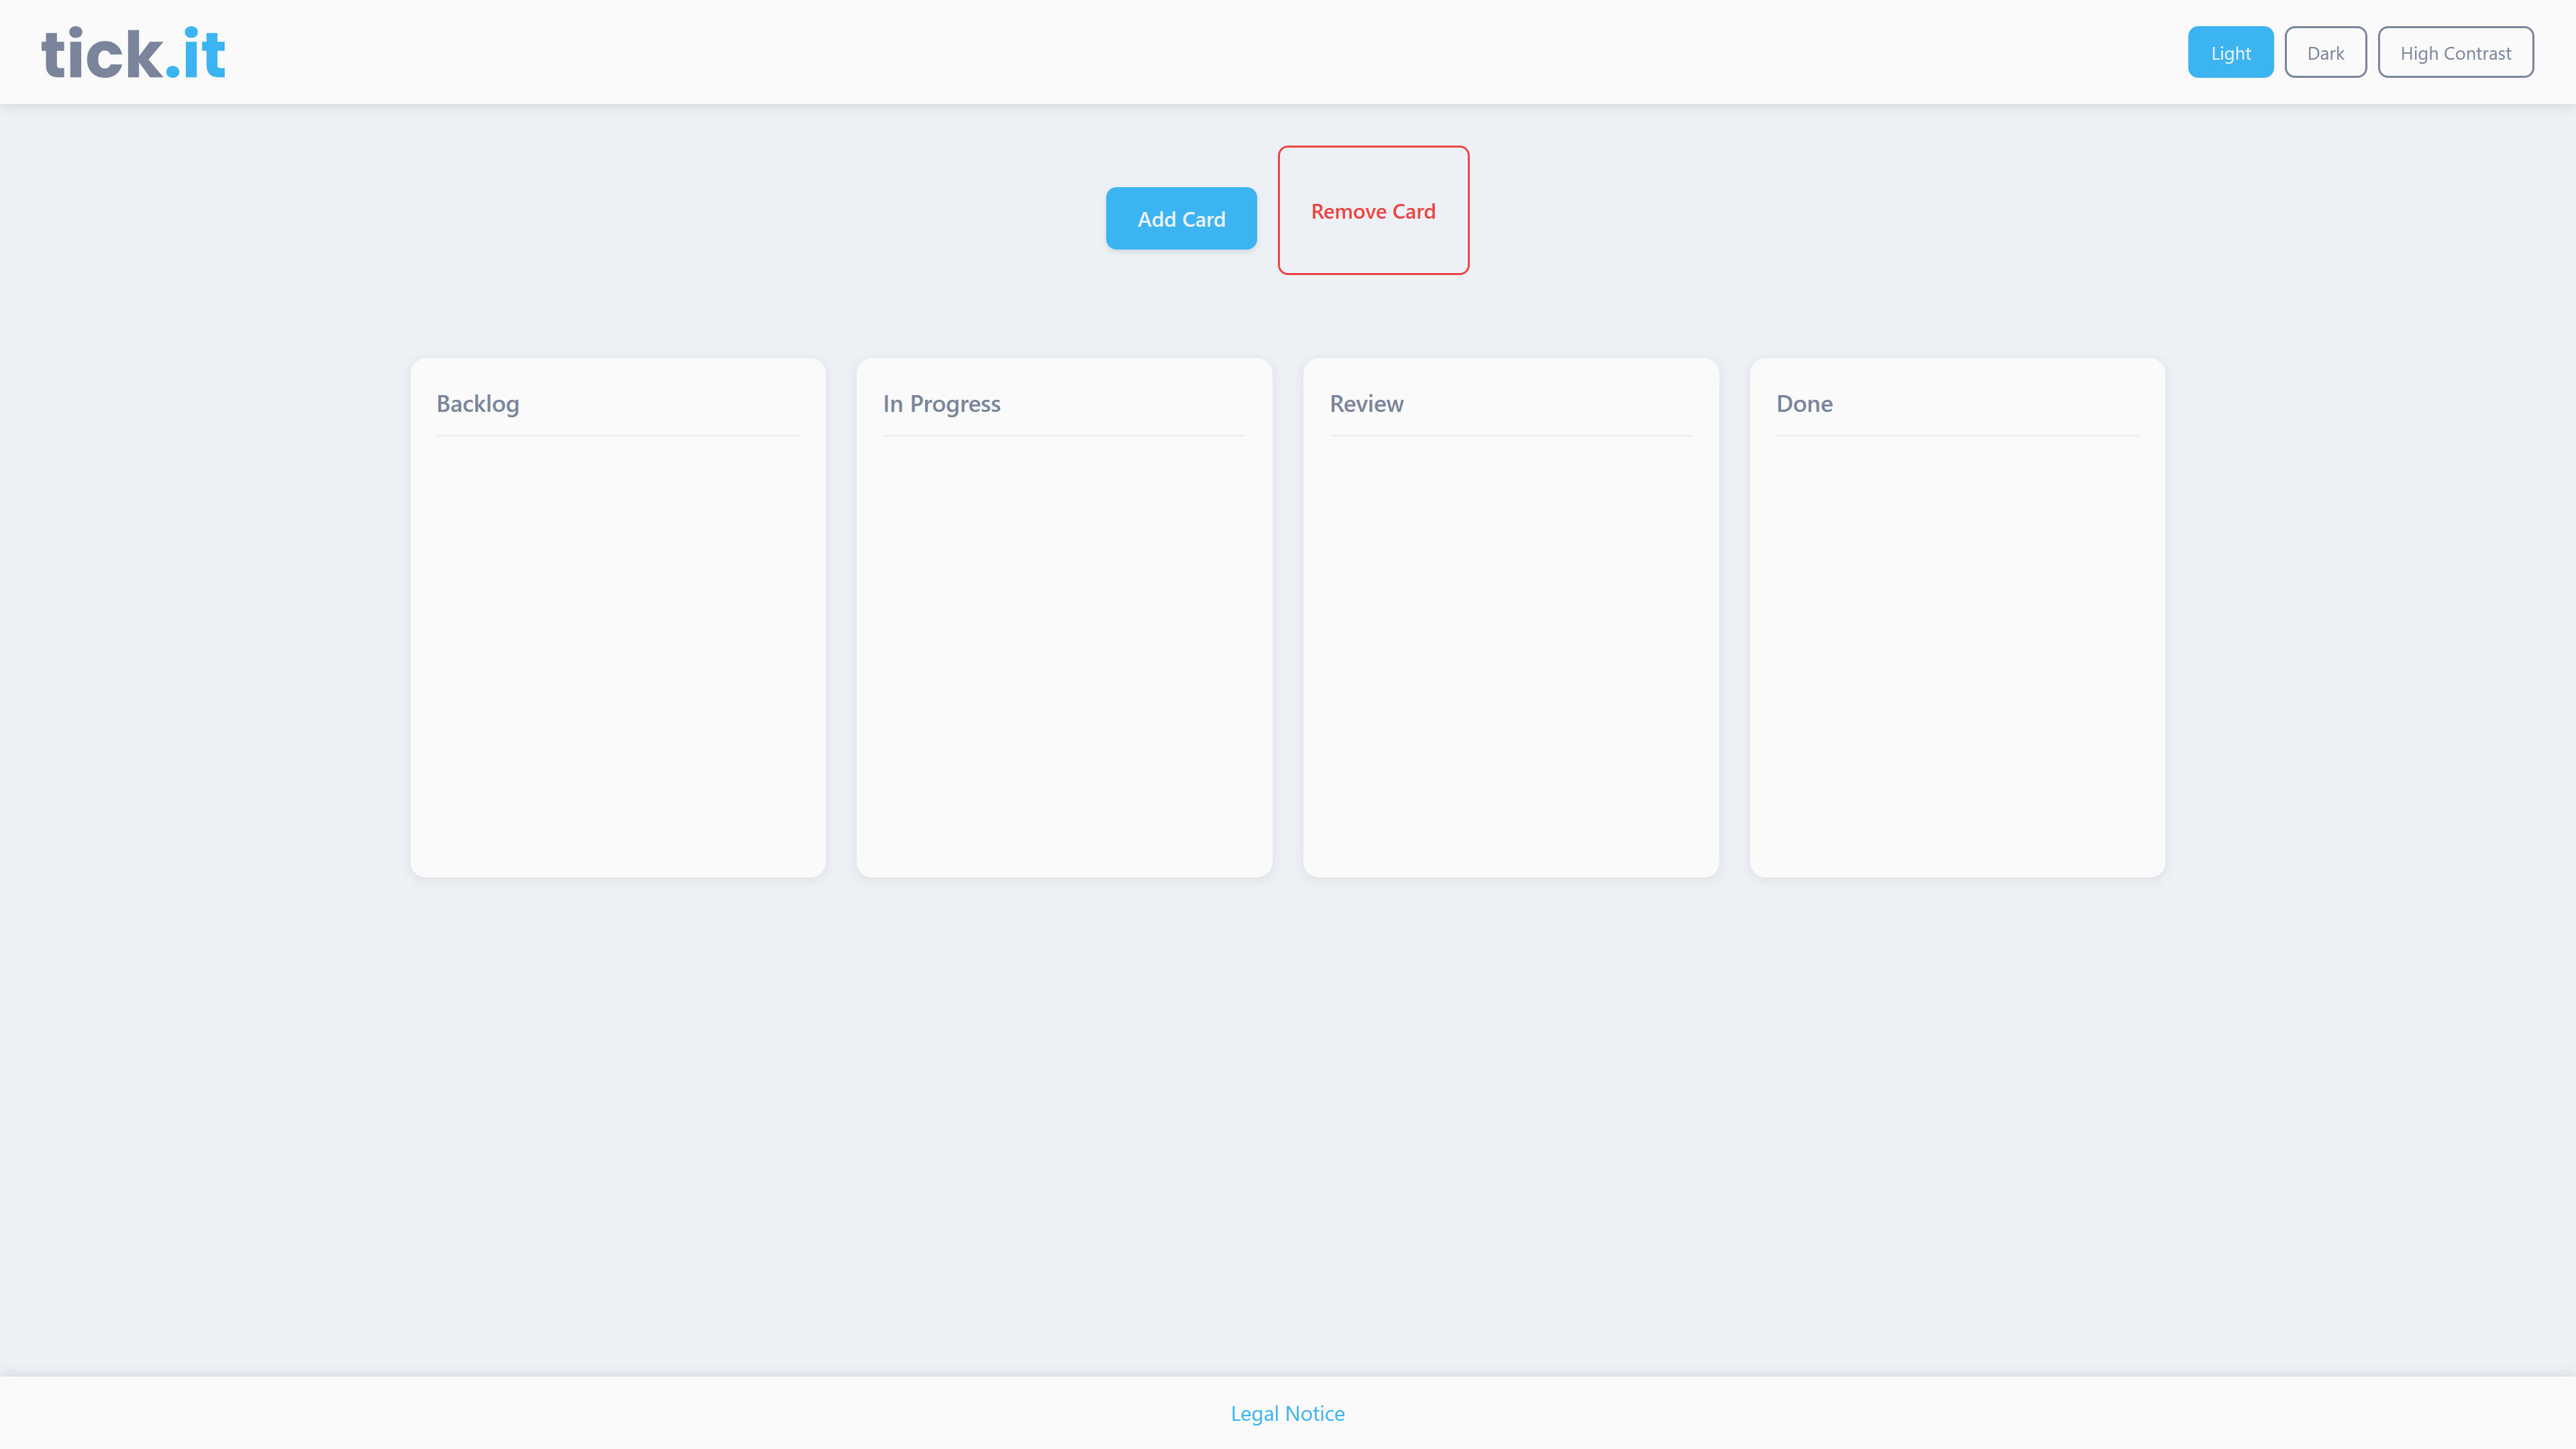
\includegraphics[width=1.0\linewidth]{tick_it_s1.png}
  \caption{tick.it Board \bildquelle{tick-it-page}}
  \label{fig:tick_it_s1}
\end{figure}

\begin{figure}[htbp]
  \centering
  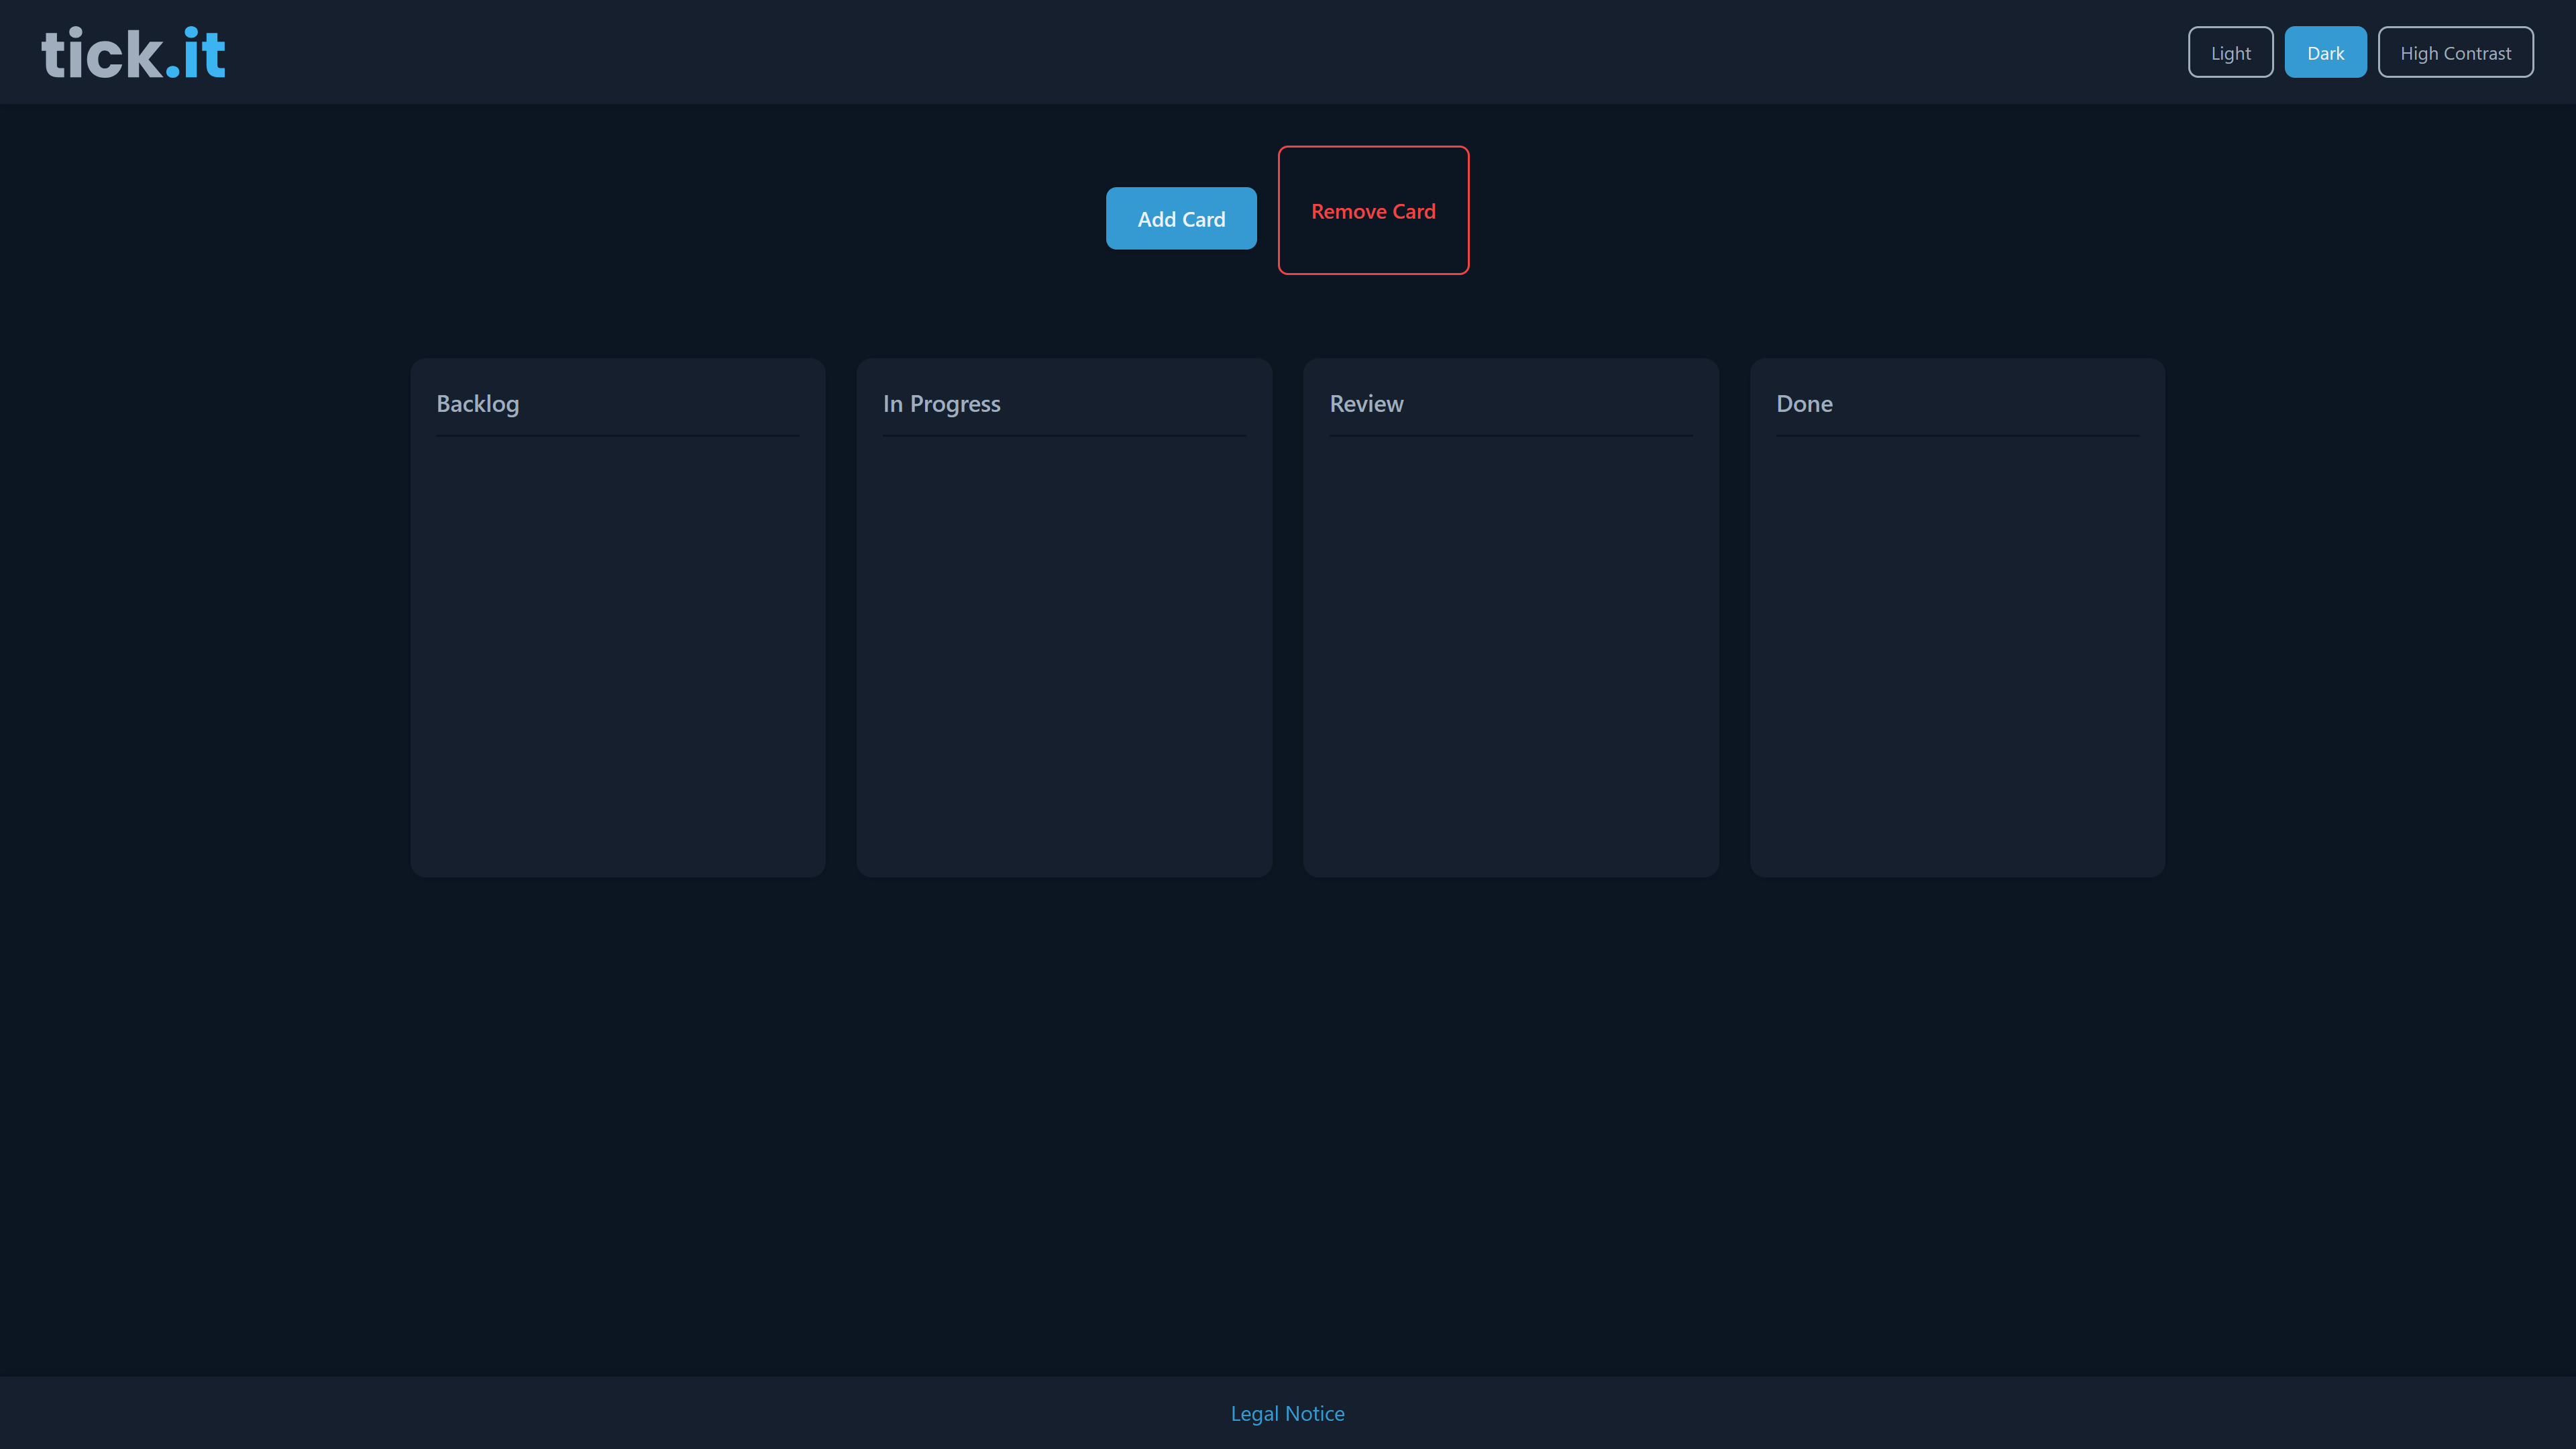
\includegraphics[width=1.0\linewidth]{tick_it_s2.png}
  \caption{tick.it Board Dark Mode \bildquelle{tick-it-page}}
  \label{fig:tick_it_s2}
\end{figure}

\begin{figure}[htbp]
  \centering
  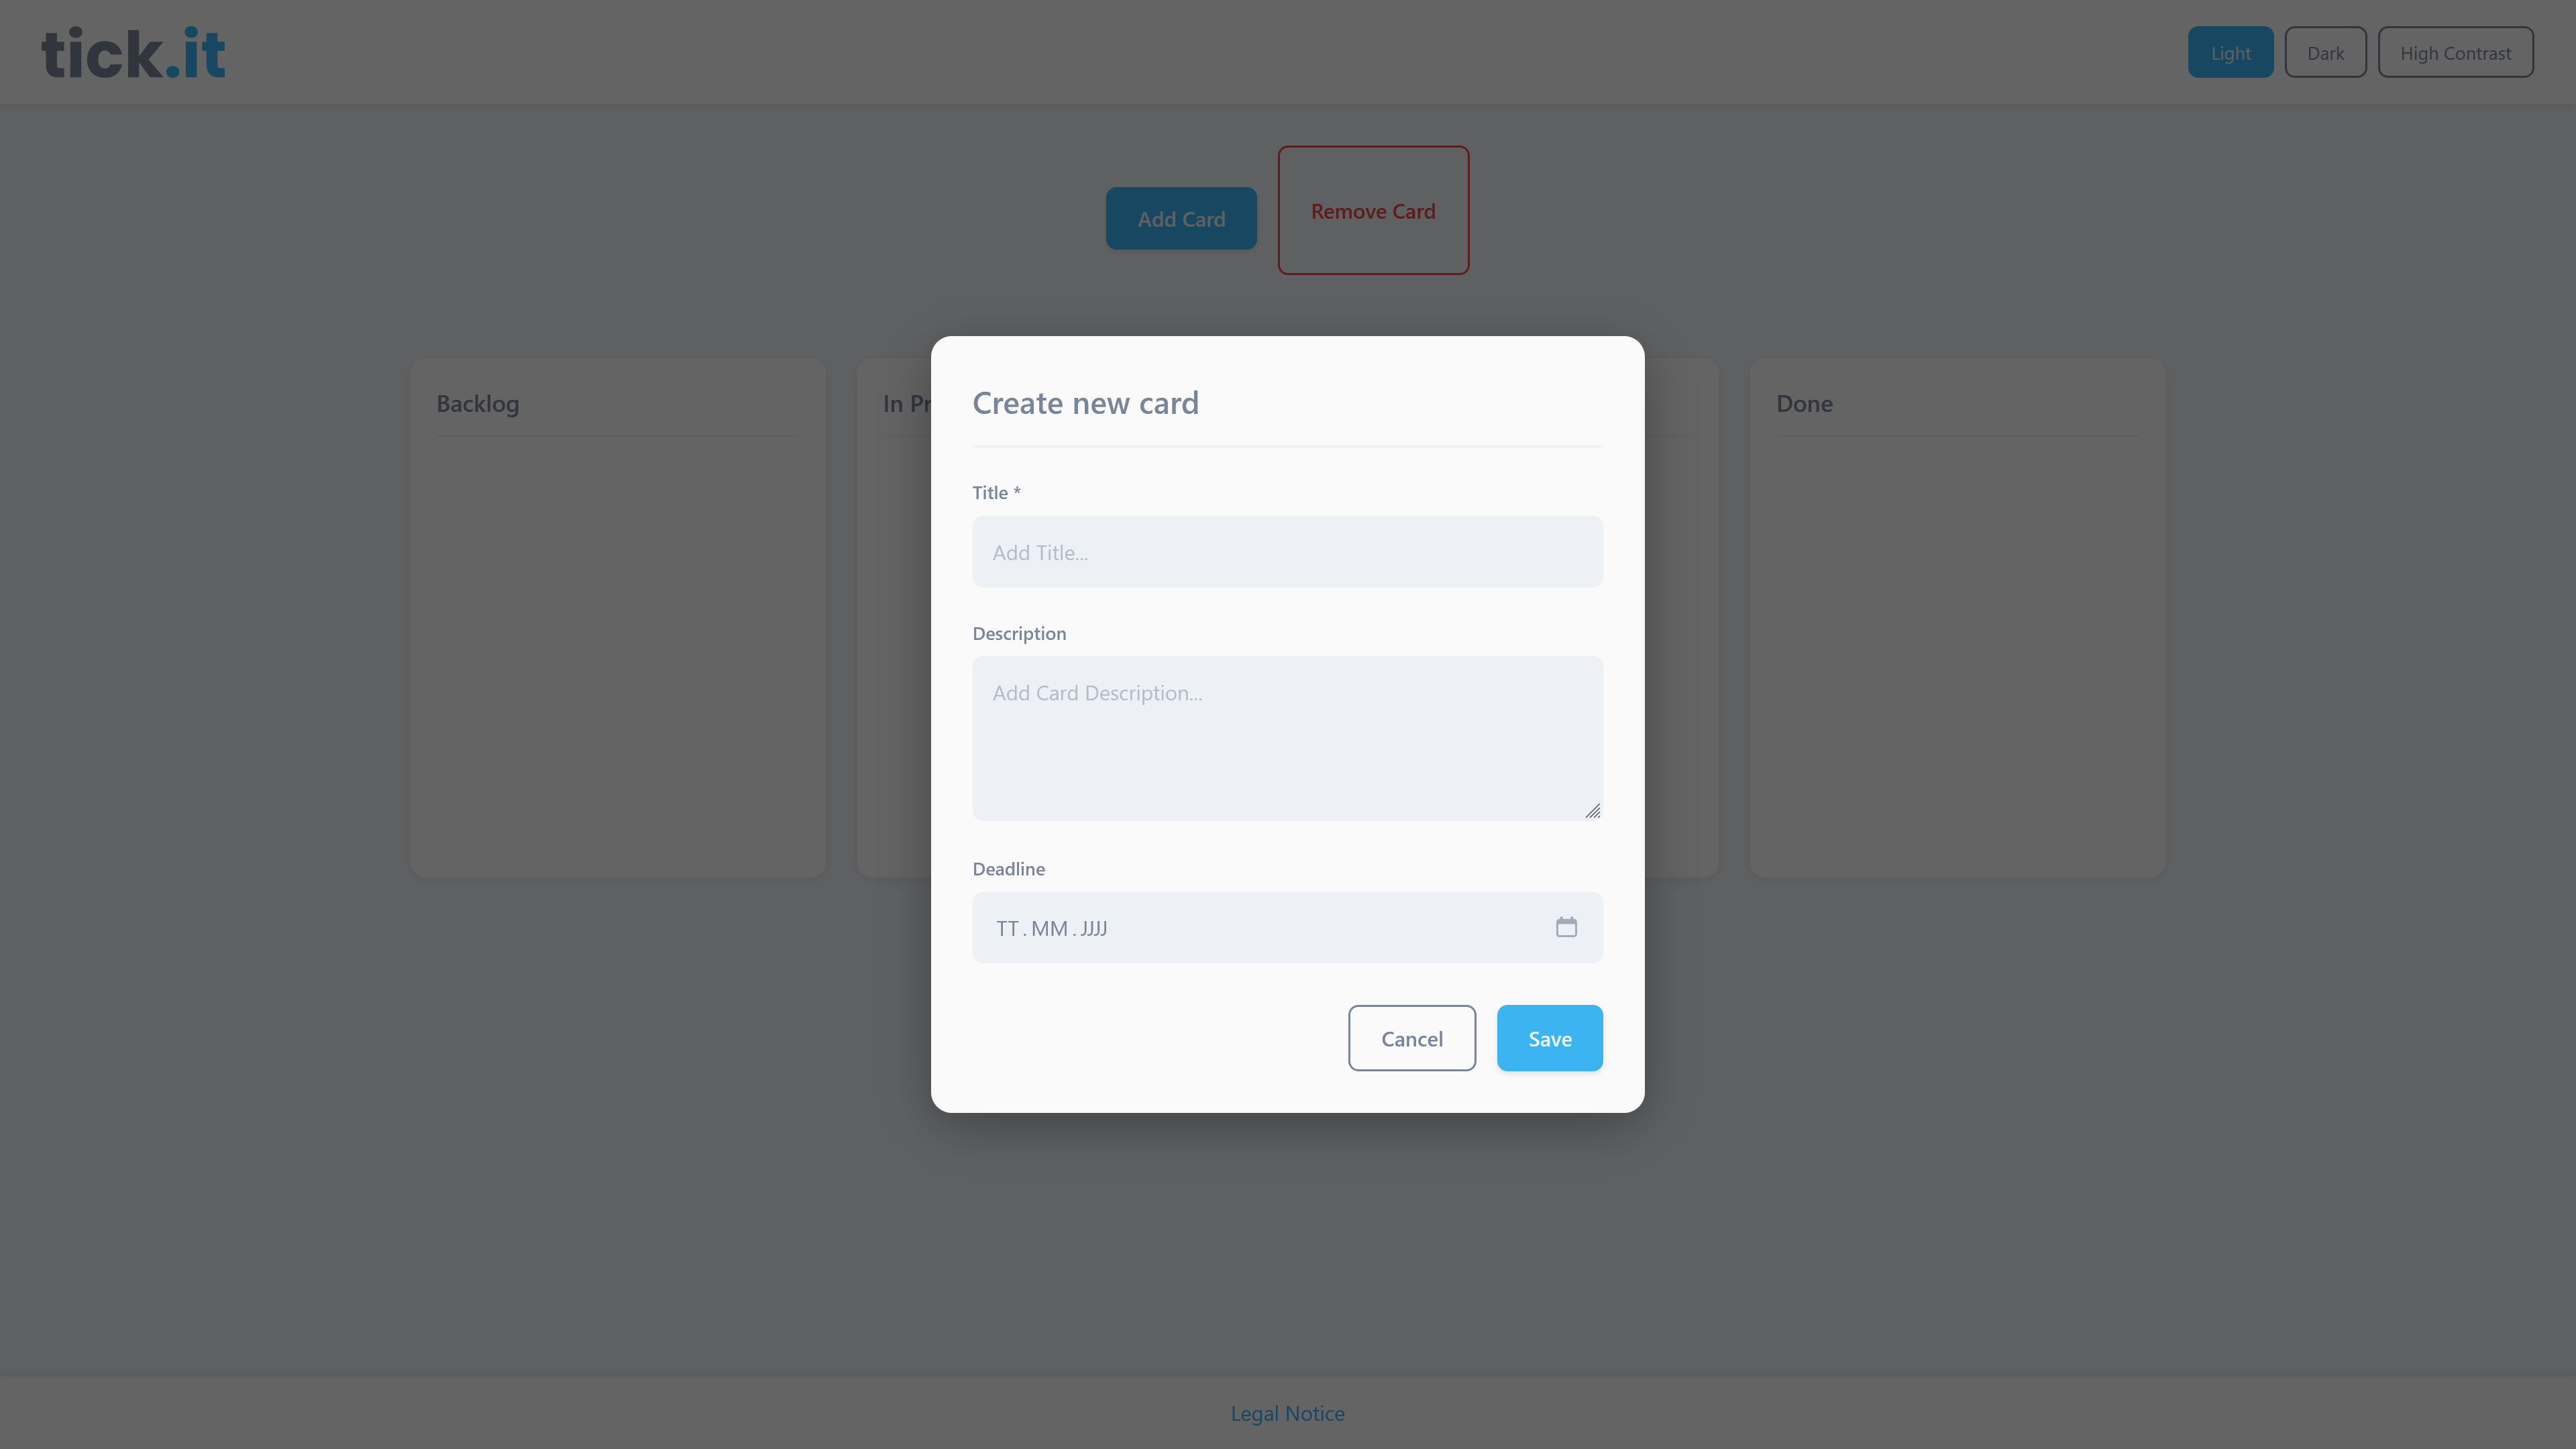
\includegraphics[width=1.0\linewidth]{tick_it_s3.png}
  \caption{tick.it Board Kartenerstellung \bildquelle{tick-it-page}}
  \label{fig:tick_it_s3}
\end{figure}


% ---------------------------------------------------------------------
\begin{beitraege}
  Text \cref{sec:pt-einleitung}                                        & Lara Senger \\
  Anlegen des Projektes & Philipp Wisser \\
  Screenshots \cref{sec:pt-screenshots} & Philipp Wisser \\
  Korrekturlesen & Tara Dethlefsen \\
  \midrule
  KI/Automatisierung: Claude Opus 5.5 zur Erstellung des LaTeX Templates \parencite{claude2026}        & Philipp Wisser \\
\end{beitraege}

%% =====================================================================
%  Aufgabe 2
% =====================================================================
\chapter{Formative Evaluation}
\label{chap:formative_evalutation}

\section{Einleitung}
\label{sec:pt-einleitung2}

Mit der formativen Evaluation wollen wir herausfinden, wie wir tick.it weiterentwickeln können, um die Anwendung auf die Bedürfnisse von Studierenden anzupassen. Wir verfolgen bei der Evaluation die folgenden drei Forschungsfragen:

\begin{enumerate}
    \item[\textbf{FF1}] Wie organisieren Studierende ihre Aufgaben mit digitalen Tools und welche Schwierigkeiten erleben sie dabei?
    \item[\textbf{FF2}] Wie erleben Studierende die Bearbeitung eines einfachen Organisationsszenarios in tick.it und welche Stärken und Probleme zeigen sich dabei?
    \item[\textbf{FF3}] Welche Anforderungen stellen Studierende an ein kollaboratives Tool zur Organisation von Gruppenarbeit?
\end{enumerate}

Unsere primäre Zielgruppe sind Studierende, die ihren Studienalltag organisieren möchten. Aus diesem Grund setzen wir für die Teilnahme voraus, dass die Personen aktuell in einem Studiengang eingeschrieben sind. Zusätzlich erfassen wir zu Beginn des Interviews vier Eigenschaften, um die Aussagen später einordnen zu können. Das Fachsemester gibt Aufschluss darüber, wie viel Erfahrung die Teilnehmenden mit der Organisation ihres Studiums im Allgemeinen haben. Die bisherige Nutzung digitaler Organisationstools ermöglicht es, ihre Erfahrung mit solchen Tools einzuordnen. Ob im Semester mehrere Aufgaben parallel anfallen, ist relevant, da die Bearbeitung mehrerer Aufgaben ein Kernszenario eines Kanban-Boards darstellt. Zudem erfassen wir, wie häufig die Teilnehmenden in Gruppen arbeiten, um ihre Aussagen zu den Anforderungen an ein kollaboratives Organisationstool einordnen zu können.

Mit dem Ziel die Bedürfnisse der Nutzenden tiefer zu verstehen, führen wir eine thematische Analyse der Interviews durch. Da die Interviews qualitative Daten liefern, die Perspektiven und Erfahrungen der Teilnehmenden abbilden, eignet sich diese Methode besonders gut. Sie ist zudem offen genug, um auch unerwartete Themen zu erfassen, die wir mit einem vorab festgelegten Kategoriensystem übersehen könnten.


\section{Vorgehen}
\label{sec:pt-vorgehen}

NOTIZEN:
Zur Beantwortung der Forschungsfragen führen wir halbstrukturierte Interviews durch. Sie eignen sich, um Erfahrungen, Schwierigkeiten und Bedürfnisse der Teilnehmenden offen zu erfassen. Zusätzlich bearbeiten die Teilnehmenden eine konkrete Aufgabe in tick.it und sprechen dabei ihre Gedanken laut aus. So verbinden wir allgemeine Erfahrungen mit dem Eindruck aus der tatsächlichen Nutzung des Prototyps und können Stärken und Probleme direkt am Szenario beobachten.
Die Interviews wurden mit Whisper (OpenAI, 2025; Radford et al., 2023), Modell medium, lokal auf einem eigenen Rechner automatisch transkribiert, sodass keine Audiodaten an externe Server übertragen wurden. Anschließend wurden die Transkripte manuell anhand der Audioaufnahmen geprüft und korrigiert sowie nach den Transkriptionsregeln überarbeitet."

% ---------------------------------------------------------------------
\begin{beitraege}
  Text \cref{sec:pt-einleitung2}  & Tara Dethlefsen \\
  \midrule
  KI/Automatisierung: keine        & -- \\
\end{beitraege}


\listoffigures
\listoftables
\printbibliography[title={Quellenverzeichnis}]

\end{document}
